\chapter{Tools and Technologies}
\label{ch:tools_technologies}
\section{FPGA \& Tools}
The FPGA development board used by this project is the Nexys-A7-100t\footnote{https://digilent.com/reference/programmable-logic/nexys-a7/start}. This development board uses the XC7A100T FPGA chip, with 128MiB of external RAM, a large array of IO ports and onboard peripherals. The FPGA chip contains 63400 LUTs, 126800 flip-flops, 2860Kb of block RAM and 240 DSP slices\cite{nexys-a7-100t}. This should be adequate for the design of a small SoC, as explained in \ref{rocketchip}, but there is risk that this won't be the case. As such, an alternative FPGA development board has been identified as the Nexys-Video\footnote{https://digilent.com/reference/programmable-logic/nexys-video/start}. This uses the XC7A200T FPGA chip, with 134600 LUTs, 269200 flip-flops, 13Mb of block RAM and 740 DSP slices\cite{nexys-video}, and will definitely be adequate for our use case.

Connection to the FPGA development board will be made using USB serial and minicom\cite{minicom}, a basic serial interaction terminal program.

Once HDL has been generated for the SoC, we need to generate the bitstream to implement it on the FPGA. We will be using Vivado for this, a software suite for design, simulation, analysis, synthesis and implementation of digital circuits using HDL. Vivado has been chosen because of our familiarity with the software, and the availability of the software to us.

\section{RocketChip} % should maybe be in background?
\label{rocketchip}
The aim of the project is to design a fully functioning RISC-V SoC that could potentially run a full OS, and attempting this from nothing would take much longer than the project timeline and is beyond the current skills of the author. Therefore, an SoC generator will be used, where we can create configuration files and semi-custom designs using high-level descriptions that have the full HDL created by software. We need a full SoC to be generated, not just CPUs, to include IO controllers, cache and other necessary components for a full computing system. Due to how niche RISC-V currently is, there is only one suitable candidate: RocketChip\cite{rocketchip}.

The RocketChip generator is a collection of smaller sub-generators that create parameterised components. These components fit together to create the full SoC via standard interfaces, allowing any design implementing the interfaces to be easily exchanged for another in the design. The most important to this project is the core, and RocketChip can generate three core types: RocketCore, BOOM\cite{boom-core} and Z-scale Core. RocketCore and BOOM are both parameterisable, allowing a semi-custom design to be created. The default BOOM core (RV64GC) utilises around 148500 LUTs for a single core, and so cannot be used with the available FPGA. A default RocketCore (RV64GC) uses approximately 38300 LUTs for a single core, and 27500 for each default core after, giving 65800 LUTs necessary for a dual core design. This is greater than the number of LUTs in the FPGA, and so we will have to design cores smaller than these defaults. Exact details of the parameterisation options available in RocketCore are in the \ref{ch:hw_design} chapter.

CPUs instantiated in a RocketChip SoC are inside of 'tiles' following the TileLink architecture\cite{tilelink}. This contains them inside standard interface sections and allows CPUs to be added to the same bus with cache coherency between all cores, as can be seen in figure \ref{fig:rocketchip_example}.

\begin{figure}[h!]
    \centering
    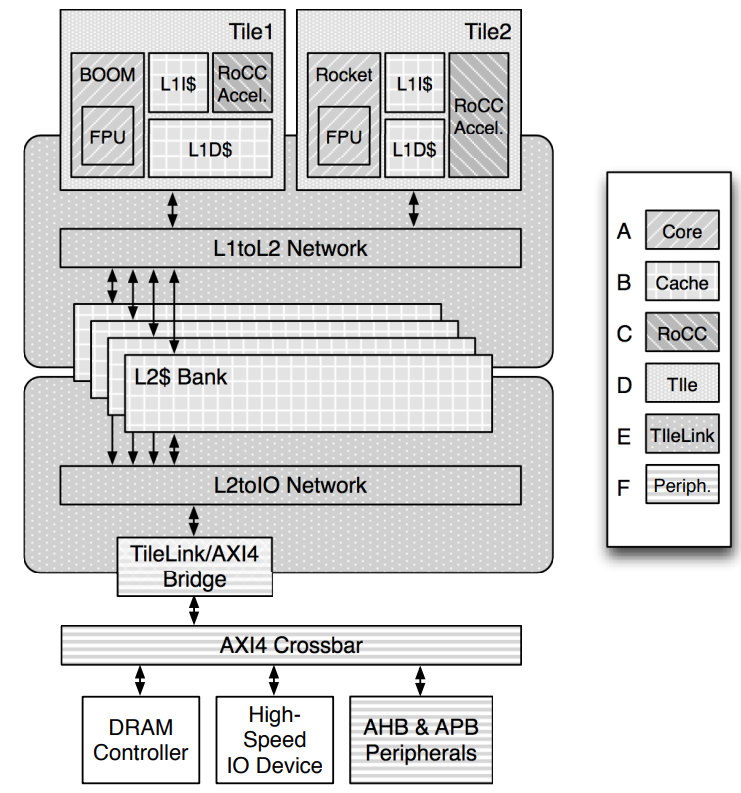
\includegraphics[width=0.7\textwidth]{img/rocketchip_soc.png}
    \caption{The layout of a RocketChip SoC with a BOOM and RocketCore\cite{rocketchip}}
    \label{fig:rocketchip_example}
\end{figure}

The RocketCore itself is a 6-stage pipelined processor with in-order issue and execution, implementing up to the RV64GC ISA. Without extensions (RV64I), the RocketCore processor has a single pipeline. Adding the floating point unit introduces the FP pipeline which runs in tandem with the integer pipeline, but only a single instruction can be issued to either the integer or floating point pipelines at once.

\begin{figure}
    \centering
    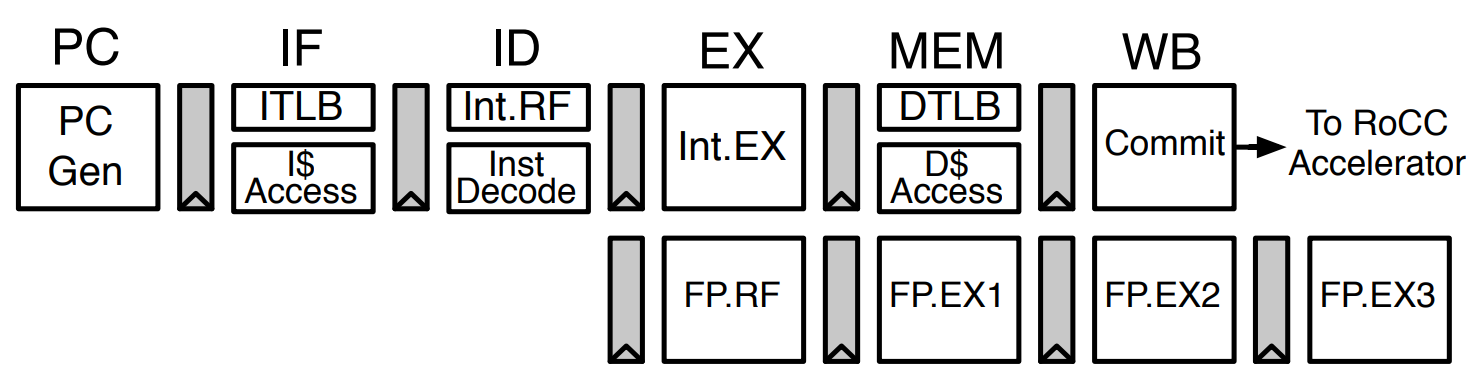
\includegraphics[width=0.9\textwidth]{img/rocketcore_pipeline.png}
    \caption{RocketCore pipeline with optional FPU\cite{rocketchip}}
    \label{fig:rocketcore_pipeline}
\end{figure}

\section{vivado-risc-v}
\label{vivado-risc-v}
This projects extends an existing repository vivado-risc-v\cite{vivado-risc-v}. The vivado-risc-v repository is a collection of other tools and resources, along with additional scripts and sources, that can generate HDL (hardware description language) for RISC-V based SoCs, link them to hardware resources on specific FPGAs using Vivado and create the bitstream to program the FPGA. The repository also has scripts to generate a bootable external memory device, such as an SD card, with OpenSBI, U-Boot, Linux kernel and Debian OS. This allows a functional RISC-V SoC to be instantiated on an FPGA, boot into Debian Linux and be used as a general-purpose computer, albeit without GUI support. The Nexys-A7-100t is directly supported by vivado-risc-v, so no changes had to be made to add support for the chosen FPGA board.

The main use of vivado-risc-v is board support and Vivado project generation. The HDL for the design is generated by the external tools, for example RocketChip to generate the SoC, sifive-cache to add more cache and testchipip for clocks, and the vivado-risc-v scripts add these to a new Vivado project setup for the FPGA board in use. vivado-risc-v also contains board-specific drivers for ethernet, SD card readers, serial connections and the device tree structure data for each board. These are necessary to connect the implemented SoC on the FPGA to the rest of the hardware on the development board.

\section{Chisel}
\label{chisel}
RocketChip is written in Chisel\footnote{https://www.chisel-lang.org/}, an open-source Scala-based HDL\cite{chisel}. Chisel describes synthesisable circuits in the same layout and precision as traditional HDLs, but with the full capabilities of the functional Scala programming language. This allows circuits to be described using functional and object-orientated methods, such as classes and recursive functions. Other beneficial features of Scala are the type system, inference of widths and data types, libraries and control flow that can change which sections of logic are used when generating the output Verilog. The output Verilog is synthesisable for FPGAs.

\section{Bare-metal code}
Once the SoC is implemented, the project aims to analyse the performance against homogeneous designs. As such, a testing suite needs to be developed to measure various performance metrics, running as bare-metal code. Bare-metal involves running as the only program on the system other than the bootloader - this means there is no OS to manage memory, threads, files and others. The code must also be written in a language than can be directly compiled to machine or byte-code, eliminating language such as Python or Java which are interpreted or run on a virtual machine. The languages with most support for RISC-V bare-metal are C/C++ and Rust, as these are often used for embedded programming. Another option is to write RISC-V assembly directly. This would make compilation much simpler, but prevents the use of libraries and is much harder to write complex programs - though it is likely the testing suite will be quite simple in order to accurately measure individual characteristics of the SoC.

\begin{description}
    \item[Rust] High-level language with speed comparable to C, memory/thread safety and excellent type system. Very detailed compiler messages and has a lot of features that would not be utilised in this usecase. Relatively easy to compile to RISC-V byte code, with crates (libraries) for low-level RISC-V programming.
    \item[C++] High-level language also with speed comparable to C. Also has many features that wouldn't be used for our purpose, similarly easy to compile to RISC-V byte code and has libraries for low-level RISC-V programming.
    \item[C] Low-level language, very fast. Has easy direct memory manipulation, easy to compile to RISC-V byte code and has similar libraries to C++ for low-level RISC-V programming.
    \item[Assembly] Byte code, will be very hard to write complex programs in but will be very easy to compile and debug in simulators by stepping through instructions individually.
\end{description}

C and Assembly are the chosen languages for the bare-metal code, due to its ease of compilation and how they can be easily mixed together. Assembly will be used to manually start the cores, jump to memory locations, etc, and C will be used to write the tests. This combination makes design and implementation of the tests easiest for the author.

Bare-metal programming will also require statically linked libraries. This means any libraries used must be compiled alongside the program and are part of the output byte code. Typical library usage is dynamically linked, where the compiled program references code in libraries that are identified when the program begins, and are loaded then. This is much harder to achieve in bare-metal, and reduces the portability of the final output.

\section{Linux}
Some of the software for the design and implementation of the SoC is only available on Linux. As such, a Linux install needs to be set up on the author's computer. We first attempted an install using windows subsystem for Linux, allowing Linux to be run semi-natively inside of Windows. This did not function as expected however, limiting the RAM available to 8GB and requiring interactions between Windows and Linux software, as well as reducing the overall performance due to extra overhead from windows. This made a large impact when doing synthesis and place and route, which are very computationally heavy tasks. We therefore installed Linux natively, solving the compatibility issues and increasing performance.

\section{Git}
Git will be used for version control of the project. Version control is highly necessary, storing historical versions of the project and allowing multiple branches of the current state to test new features in isolation of other developments. GitHub is used as a remote repository, a backup of the project. This will also allow development to be synchronised across multiple devices, beneficial as work will be completed by the author in a multitude of places.